\chapter{Material und Methoden}
\label{chap.material}
\prever{
%Anwendung nicht als System zur detektion der Projektion, sondern als gekoppeltes System. Dadurch Lichtstärke nur für den Anwender relevant, nicht aber für die Erkennung von Strukturen o.ä.\\
%\kps{} auslagern oder in Material beschreiben?\\
%\kps{} Kalibrierung etc. inkl. Grundlagenteil, wie ausführlich?\\
%GUI Struktur auslagern oder hier beschreiben?\\
\red[TODO:\\
Blockschaltbild zu technischen Komponenten\\
Blockschaltbild Software Elemente gleiche Form!?\\
Notation verschieben\\
KS für Bildebene einführen!?\\
]
}
Dieses Kapitel erläutert die Elemente, aus welchen das erstellte \kps{} aufgebaut wurde. Neben den verwendeten technischen Komponenten wird die Kalibrierung des \kps{s} beschrieben. Darüber hinaus erfolgt eine Darstellung der verwendeten Softwarebibliotheken und der entwickelten Programmstruktur.

\section{Technische Komponenten}
Das erstellte System wurde aus verschiedenen Komponenten aufgebaut, welche im Folgenden näher beschrieben werden sollen. 
\prever{
%\red[TODO: PC Beschreibung]
}
\subsection{Microsoft Kinect\textsuperscript{\texttrademark} Sensor}
\label{chap.kinect}
Der von Microsoft (Microsoft Corporation, Redmond, USA) entwickelte Kinect\textsuperscript{\texttrademark} Sensor\footnote{Im Folgenden als Kinect bezeichnet.} ist ein System, welches eine natürliche Benutzerschnittstelle für Computer und Spielkonsolen bereitstellt. Es ermöglicht die Steuerung von Programmen und Spielen durch Gesten, Körperbewegungen und Sprachbefehle. Die Kinect verfügt über zwei Kameras, mit denen Videoaufnahmen im Farb- (RGB) sowie im Infrarotbereich (IR) möglich sind. Die Technik zur Ermittlung der Tiefeninformationen stammt von der Firma PrimeSense (PrimeSense LTD, Tel Aviv, Israel) und ist unter anderem durch das Patent \cite{Freedman2008} geschützt. Die IR-Kamera wird dabei in Verbindung mit einem IR-Projektor verwendet, um Tiefenbilder zu generieren. Der IR-Projektor projiziert ein irreguläres, bekanntes Muster, welches von der IR-Kamera erkannt wird. Über die Verzerrungen des Musters sind anschließend softwareseitig Rückschlüsse auf die Tiefenwerte der aufgenommenen Szene möglich. Da ein Projektor auch als inverse Kamera betrachtet werden kann \cite{Kimura2007}, entspricht der Aufbau der Kinect dem einer Stereokamera. Die Bildachsen der IR-Kamera und des IR-Projektors sind parallel orientiert, so dass ein Punkt $\vec{P}$ im projizierten Muster auf der in \abb{fig.kinect_depth} dargestellten horizontalen Epipolarlinie $\vec{e}$ in der Bildebene der Kamera abgebildet wird.\\

\nomenclature[a]{RGB}{Farbraum, beschrieben durch die Grundfarben Rot, Grün und Blau}
\nomenclature[a]{IR}{Infrarot}

\begin{figure}[ht]
	\begin{center}
		\includesvgnew[1]{images/epipolar_3d_04}
		%
\includegraphics[scale=1.0]{spacer}
		\caption{Bestimmung des Tiefenwertes eines Punktes über die Epipolargeometrie am Beispiel der Kinect}
		\label{fig.kinect_depth}
	\end{center}
	%\vspace*{-8mm}
\end{figure}

\prever{
%\red[Bildebenen kennzeichnen\\Beschreiben, dass Bildebenen dargestellt sind\\]
}

Wird der korrespondierende Punkt im Kamerabild identifiziert, kann die Disparität $d = x - x'$ berechnet und zusammen mit dem Basisabstand $D$ und der Brennweite $f$ darüber der Tiefenwert des Punktes bestimmt werden:
%
\nomenclature[l]{$d$}{Disparität}
\nomenclature[l]{$D$}{Basisabstand der Bildachsen von IR-Kamera und -Projektor der Kinect}
\nomenclature[l]{$f$}{Brennweite}
\nomenclature[l]{$\vec{e}$}{Epipolarlinie}
%\nomenclature[l]{$z$}{Tiefenabstand eines Punktes im Koordinatensystem der Kinect}
%
%
\begin{equation}
z = \frac{D}{d}\cdot f
\end{equation}

Die bekannte relative Pose zwischen der RGB- und IR-Kamera ermöglicht abschließend die Zuordnung von Farb- und Tiefenwerten (englisch Depth Values). Sensoren dieser Art werden daher auch als RGB-D Kameras bezeichnet.\\

\nomenclature[a]{RGB-D}{Ergänzung des abgebildeten Farbraums um Tiefeninformationen}

Die Kinect stellt eine kostengünstige Möglichkeit zur simultanen Aufnahme von Tiefen- und Farbinformationen dar. Da seit der Veröffentlichung verschiedene quelloffene Treiber entwickelt wurden, eignet sich die Kinect besonders für die Anwendung in der Forschung. In dieser Arbeit werden neben den Daten der RGB-Kamera auch die Tiefeninformationen sowie die daraus generierten Punktwolken\footnote{Punktwolken sind Datenstrukturen, welche eine Sammlung multidimensionaler Punkte repräsentieren.
%Als Punktwolke wird die Repräsentation der Tiefenwerte durch eine Menge aus Punkten mit dreidimensionalen Koordinaten bezeichnet.
} verwendet.

%Die Kinect umfasst über die Kamerasysteme hinaus vier Mikrofone zur Sprachsteuerung und einen Motor, welcher die Veränderung des Neigungswinkels ermöglicht. Diese Funktionen sind jedoch nicht Bestandteil des in dieser Arbeit entwickelten Systems.\\

%\red[Da Microsoft selbst keine Angaben über die von ihnen lizensierte Technologie macht stammen die Beschreibungen zur Funktionsweise der Kinect aus den Patentschriften der Firma PrimeSense.]\\

\prever{
%\red[Datenblatt/Spezifikationen in Anhang!\\]
}

\subsection{Microvision ShowWX+\textsuperscript{\texttrademark}}%Pico Laser Projektor}
\label{chap.projector}
Der Pico-Laser-Projektor ShowWX+\textsuperscript{\texttrademark} der Firma Microvision (Microvison Inc., Redmond, USA) zeichnet sich neben der geringen Größe dadurch aus, dass als Lichtquellen drei Laser in den Farben rot, grün und blau eingesetzt werden. Die Strahlen werden wie in \abb{fig.projtech} gezeigt durch Optiken kombiniert, um alle Farben des sichtbaren Spektrums abzubilden. Der Bildaufbau erfolgt durch Ablenkung des kombinierten Strahls an einem MEMS\footnote{Ein MEMS (Mikro-elektromechanisches System) ist ein technisches System, welches aus Komponenten aufgebaut ist, deren Abmessungen im Mikrometerbereich liegen.}-Spiegel mit zwei Freiheitsgraden.

\nomenclature[a]{MEMS}{Mikro-elektromechanisches System}

\begin{figure}[ht]
	\begin{center}
		\includesvgnew[1]{images/projector_tech_03}
%		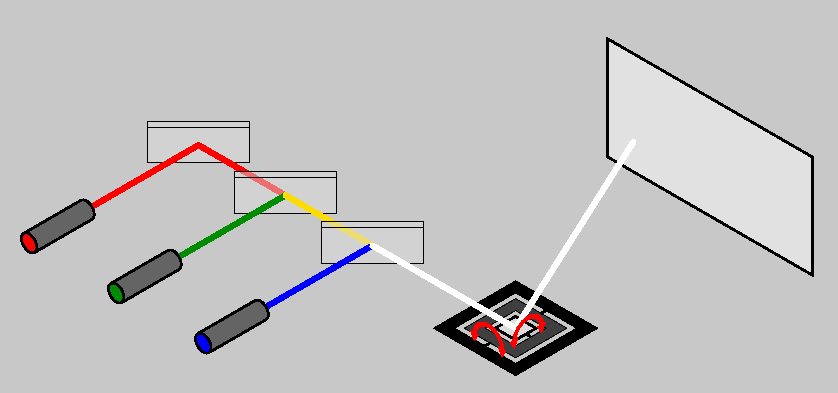
\includegraphics[scale=1.0]{projector_tech_02}
		\caption{Projektionsprinzip des Pico-Laser-Projektors}
		\label{fig.projtech}
	\end{center}
	%\vspace*{-8mm}
\end{figure}

\prever{
%\red[Laser ergänzen]
}

Die Verwendung von Lasern führt dazu, dass die Schärfe des Bildes unabhängig vom Abstand zur Projektionsfläche ist. Der Einsatz von Linsen zur Fokussierung der Strahlen ist daher ebenso wie eine manuelle Anpassung der Fokuseinstellungen nicht erforderlich. Genauere Spezifikationen des ShowWX+\textsuperscript{\texttrademark} finden sich in Anhang \ref{app:projector}.


\subsection{Arduino\textsuperscript{\texttrademark} Nano}
\label{chap.arduino}
Der Arduino\textsuperscript{\texttrademark} Nano\footnote{Im Folgenden als Arduino bezeichnet.} ist ein quelloffenes Mikrocontroller Board, welches durch Schnittstellen in Form von analogen und digitalen Ein- und Ausgängen die Steuerung, Kontrolle und Kommunikation mit elektronischen Komponenten wie Sensoren oder Aktoren ermöglicht. Eine detaillierte Auflistung der Spezifikationen des Arduino findet sich in \anhang{app:arduino}. Die zur Erstellung von Programmen bereitgestellte, ebenfalls quell-offene, Software bildet im Zusammenhang mit der Hardware eine ganzheitliche Entwicklungsumgebung, mittels derer sich Projekte unterschiedlicher Komplexität realisieren lassen. Der Arduino verfügt über eine USB-Schnittstelle, welche sowohl die Übertragung der erstellten Software auf den Arduino, als auch den Empfang von Kommunikationsdaten ermöglicht. Damit zusätzliche Informationen für die Lokalisation des \kps{s} zur Verfügung gestellt werden können, wird der Arduino in dieser Arbeit verwendet, um eine inertiale Messeinheit in das System zu integrieren.

\prever{
%\red[Auf Berechnung der Lagedaten näher eingehen?]\\
%\red[Buttons eingebaut, kurz ansprechen hier]
}

%\cite{http://arduino.cc/en/Main/ArduinoBoardNano}

\subsection{Inertiale Messeinheit}
\label{chap.imu}
Die von der Firma InvenSense (InvenSense Inc., San Jos\'e, USA) entwickelte inertiale Messeinheit (englisch Inertial Measurement Unit, IMU) MPU-9250 ermöglicht die Messung von Beschleunigungsdaten bezüglich der sechs räumlichen Freiheitsgrade des Systems. Aus diesen Daten kann die Orientierung des Systems bezüglich der Achswinkel bestimmt werden \cite{IMU}. Die Anbindung an das System erfolgt wie zuvor beschrieben durch den Arduino, welcher wiederum die Schnittstelle zu der entwickelten Programmstruktur bildet.
\prever{
%\red[Datenblatt in Anhang!]
}

%Kompass hier nicht verwendet, aber spätere Verwendung denkbar, bedeutet allerdings, dass Orientierung des Raumes bekannt sein muss (oder irgendwie später hinzugefügt werden kann)
%\cite{http://www.invensense.com/mems/gyro/mpu6500.html}

\subsection{Raspberry Pi\textsuperscript{\texttrademark}}
Der Raspberry Pi\textsuperscript{\texttrademark} Computer\footnote{Im Folgenden als Raspberry bezeichnet.} wurde von der Raspberry Pi Foundation (Caldecote, Vereinigtes Königreich) entwickelt und ist ein ARM\footnote{ARM (Advanced RISC Machines) ist eine von der Firma ARM (ARM Limited, Cambridge, Vereinigtes Königreich) entwickelte Systemarchitektur für Mikroprozessoren, welche sich durch geringen Energiebedarf bei hoher Leistungsfähigkeit auszeichnet.}-basierter Mini-Computer, welcher auf einer einzigen Platine aufgebaut ist. Das Ziel der Entwicklung des Raspberry liegt in der Realisierung eines voll funktionsfähigen Computers mit geringen Kosten, um die Verbreitung besonders in Schulen und Bildungseinrichtungen zu ermöglichen und so das Erlernen von Programmier- und Computerkenntnissen bei Kindern und Jugendlichen zu fördern. Detaillierte Spezifikationen des Raspberry sind in \anhang{app:raspberry} aufgeführt.\\

Der Raspberry wird für diese Arbeit mit einer angepassten Version des in Kapitel \ref{chap:ros} beschriebenen Meta-Betriebssystems Robot Operating System (ROS) betrieben, um die Anbindung an die entwickelte Programmstruktur zu gewährleisten. Der Raspberry dient dabei dazu, das Signal des zu projizierenden Bildes zu empfangen und über den Projektor darzustellen. Durch die direkte Anbindung des Projektors an den Raspberry entsteht ein gekapseltes System, welches damit in jeder auf ROS basierenden Anwendung eingesetzt werden kann.

\nomenclature[a]{ARM}{Advanced RISC Machines}
\nomenclature[a]{RISC}{Reduced Instruction Set Computer}

\section{Aufbau des \kps{s}}
Aus den beschriebenen Komponenten wurde das in Bild \ref{fig.kinpro} dargestellte handführbare \kps{} aufgebaut. Die Pose des Projektors wurde dabei so gewählt, dass eine Überdeckung des Projektionsfeldes mit dem Sichtfeld der RGB-Kamera der \kin erreicht wird. Im Zentrum des Systems ist eine Leiterplatte positioniert, über welche die Kommunikationsverbindung zwischen der IMU und dem Arduino realisiert wird.\\

\begin{figure}[ht]
	\begin{center}%
		\includesvgnew[1]{images/kinpro_overview_pathes}%
%		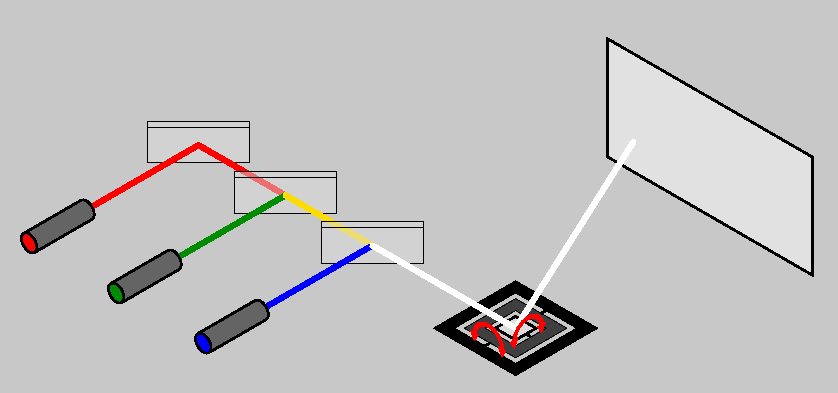
\includegraphics[scale=1.0]{projector_tech_02}
		\caption{Komponenten des aufgebauten \kps{s}}
		\label{fig.kinpro}
	\end{center}
	%\vspace*{-8mm}
\end{figure}

Die Selbstlokalisation des Systems basiert auf einem Abgleich zwischen Umgebung und Modelldaten. Voraussetzung dafür ist die Kenntnis über die Abbildungstransformation zwischen den Punkten der Umgebung und den Koordinaten der Kinect. Es wird daher eine Kalibrierung der Kameras der Kinect durchgeführt, um die Abbildungsgleichungen zu bestimmen.\\

Auch die lagerichtige Projektion in der Umgebung erfordert die Ermittlung von Koordinatentransformationen. Die Pose des Projektors kann aufgrund der Fixierung innerhalb des \kps{s} durch eine Transformation zwischen den Projektor-Koordinaten und den Kamera-Koordinaten ausgedrückt werden. Neben der Transformationsvorschrift zwischen Kamera und Projektor ist die Bestimmung der Abbildungsgleichung zwischen der Bildebene des Projektors und den Punkten der Umgebung erforderlich. Der Projektor wird wie beschrieben als inverse Kamera betrachtet, die Kalibrierung erfolgt daher basierend auf dem Vorgehen der Kamerakalibrierung. Der Ablauf der sequentiellen Kalibrierung des Gesamtsystems wird im Folgenden näher beschrieben. 
\prever{
\red[Zunächst werden dafür einige Begriffe und Notationen definiert, welche im Verlauf dieser Arbeit verwendet werden.]
}
% werden darüber hinaus weitere Transformationen bestimmt. Die extrinsische Projektor-Transformation beschreibt die Lage des Projektors bezüglich der Kamera und darüber auch bezüglich der Umgebung. Abbildungen zwischen Umgebungspunkten und Projektorkoordinaten werden über die intrinsische Projektor-Transformation charakterisiert. Bei bekannten Kalibrierungsparametern der Kamera lassen sich beide Transformationen durch eine gekoppelte Kalibrierung des \kps{s} bestimmen. 
%Um diese Transformation zu ermitteln wird eine Kalibrierung der RGB- und der IR-Kamera der Kinect durchgeführt.\\

\subsection{Begriffe und Notationen}
In Anlehnung an die Literatur \cite{Zhang2000} werden 2D-Punkte mit \pteq{x,y} und 3D-Punkte mit \pteq[P]{X,Y,Z} bezeichnet. Auf gleiche Weise werden auch Vektoren und Matrizen beschrieben, ausgenommen der für die Punktbeschreibung verwendeten Notation. Vektoren werden demnach über $\vec{v}$ und Matrizen über $\vec{M}$ beschrieben. Mittels der homogenen Koordinatendarstellung lassen sich Punkte gleichzeitig sowohl translatorisch als auch rotatorisch transformieren. Dazu wird der \textit{inverse Streckungsfaktor} $w$ als zusätzliche Komponente eingeführt, für welchen standardmäßig $w=1$ gilt \cite{Nischwitz20111}. Zur Unterscheidung werden homogene Koordinaten damit zu \ptheq{x,y} beziehungsweise \ptheq[P]{X,Y,Z} definiert. Falls nicht mittels eines vorangestellten Index $\ve{A}{p}$ anders gekennzeichnet, bezieht sich die Darstellung von Punkten und Körpern immer auf das Inertialkoordinatensystem, welches mit $\ks{0}$ bezeichnet wird. Transformationsvorschriften zwischen zwei Koordinatensystemen $\ks{A}$ und $\ks{B}$ werden mit Hilfe der Matrixschreibweise als $\tmat{B}{A}$ ausgedrückt. Die Transformation, die einen Punkt vom Inertialkoordinatensystem in das Koordinatensystem des Projektors $\ks{P}$ abbildet, lässt sich beispielsweise ausdrücken als:%
%
\begin{equation}
\ve{P}{\tilde{P}} = \tmat{P}{0}\cdot\ve{0}{\tilde{P}}
\end{equation}

\nomenclature[a]{KS}{Koordinatensystem}
\nomenclature[l]{$\vec{p}$}{Punkt in 2D-Koordinaten}
\nomenclature[l]{$\vec{P}$}{Punkt in 3D-Koordinaten}
\nomenclature[l]{$\tilde{\vec{p}}$}{Punkt in homogenen 2D-Koordinaten}
\nomenclature[l]{$\tilde{\vec{P}}$}{Punkt in homogenen 3D-Koordinaten}
\nomenclature[l]{$w$}{Inverser Streckungsfaktor}
\nomenclature[l]{$i$}{Zählvariable}
%\nomenclature[l]{$a,b$}{Variablen}
\nomenclature[l]{$\tmat{B}{A}$}{Homogene Transformation vom $\ks{A}$ ins $\ks{B}$}
%\nomenclature[l]{$\ks{j},\ks{k}$}{Variable Koordinatensysteme}
\nomenclature[k]{$\ks{0}$}{Inertialkoordinatensystem}
\nomenclature[k]{$\ks{K}$}{KS der RGB-Kamera der Kinect}
\nomenclature[k]{$\ks{K_\ind{IR}}$}{KS der IR-Kamera der Kinect}
\nomenclature[k]{$\ks{P_\ind{IR}}$}{KS des IR-Projektors der Kinect}
\nomenclature[k]{$\ks{KPS}$}{Basis-KS des \kps{s}}
\nomenclature[k]{$\ks{P}$}{KS des Pico-Laser-Projektors}
\nomenclature[k]{$\ks{M}$}{KS der Lokalisationsumgebung}
\nomenclature[k]{$\ks{Env}$}{KS der Modellumgebung}
\nomenclature[k]{$\ks{Odom}$}{Odometrie-KS für die Bewegung des \kps{s}}
\nomenclature[k]{$\ks{MF}$}{KS des Markerfeldes}
\nomenclature[k]{$\ks{K_\ind{ext}}$}{KS der externen Kamera}


Weiterhin werden die in der Literatur verbreiteten Konventionen für die Darstellung und Orientierung von Koordinatensystemen verwendet: Die farbliche Zuordnung der Koordinatenachsen richtet sich nach der RGB-Darstellung. Die $x$-Achsen werden somit rot, die $y$-Achsen grün und die $z$-Achsen blau eingefärbt abgebildet. Bei Kameras und Projektoren werden die Orientierungen der körpereigenen Koordinatensysteme so gewählt, dass die $z$-Achsen in Richtung der optischen Achsen ausgerichtet sind. Die gewählten Konventionen verdeutlicht \abb{fig.coords} anhand des \kps{s}.

\begin{figure}[ht]
	\begin{center}%
		\includesvgnew[1]{images/coordinate_systems_KS}%
		%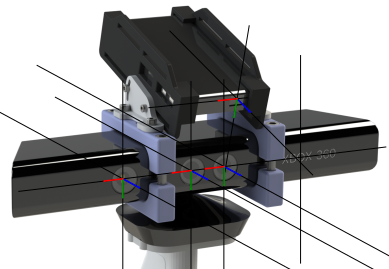
\includegraphics[scale=1.0]{coordinate_systems}
		\caption{Darstellung von Koordinatensystemen, Punkten und Transformationen am Beispiel des \kps{s}}
		\label{fig.coords}
	\end{center}
	%\vspace*{-8mm}
\end{figure}

\prever{
%\red[Punkte in KS einfügen!\\Punkte als Kreuze?\\]
%\red[Koordinatensysteme nennen!?\\]
}

\subsection{Kamerakalibrierung}
\label{chap.calib}
%Ziel der Kalibrierung ist es, die Transformation $\tmat{S}{0}$ zu bestimmen, welche die Punkte der realen Umgebung $\ve{0}{P}$ auf die Sensorkoordinaten der Kamera $\ve{S}{p}$ abbildet:
Ziel der Kalibrierung ist es, die Funktion $g$ zu bestimmen, welche die Punkte der realen Umgebung $\ve{0}{P}$ auf die Sensorkoordinaten der Kamera $\ve{S}{p}$ abbildet:
%
\begin{equation}
g : \; \ve{0}{P} \mapsto \ve{S}{p}
\end{equation}

\nomenclature[l]{$g$}{Abbildungsfunktion}

\prever{
%\red[Wie verschiedene Kameras unterscheiden, KRGB und KIR, Sensorebene: SRGB und SIR und für Projektor SP?\\]
}
Unter Verwendung des Lochkameramodells \cite{Jaehne2012}, welches von einer Kamera ohne Optik mit infinitesimal kleiner Blendenöffnung ausgeht, kann diese Abbildung beschrieben werden über:
%
\begin{equation}
s \cdot \ve{S}{\tilde{p}} = \tmat{S}{0} \cdot \ve{0}{\tilde{P}}
\label{eq.persp_abb}
\end{equation}

\nomenclature[l]{$s$}{Skalierungsfaktor}

Dabei wird über den Skalierungsfaktor $s$ die Unbestimmtheit der Tiefeninformationen beschrieben, da alle Punkte auf der Verbindungslinie zwischen $\ve{0}{\tilde{P}}$ und $\ve{S}{\tilde{p}}$ ebenfalls auf $\ve{S}{\tilde{p}}$ abgebildet werden.\\ 
\prever{
%\red[Bild, dass die Uneindeutigkeit zeigt?\\]%
}
Die Transformationsmatrix $\tmat{S}{0}$ beschreibt das Produkt aus der intrinsischen $\tmat{S}{K}$ und extrinsischen $\tmat{K}{0}$ Matrix der Kamera:
%
\begin{equation}
\tmat{S}{0} = \tmat{S}{K} \cdot \tmat{K}{0}
\end{equation}

Durch die Kamerakalibrierung können die Parameter dieser beiden Matrizen bestimmt werden. Die intrinsischen Parameter der Kamera sind konstant, während die extrinsische Kameramatrix in der späteren Anwendung durch die Lokalisation ermittelt wird. Im Rahmen der Kamerakalibrierung dient sie daher lediglich zur Bestimmung der intrinsischen Parameter. Die folgende Beschreibung des Kalibriervorgangs gilt sowohl für die RGB- als auch für die IR-Kamera der Kinect. Die Abläufe unterscheiden sich lediglich bezüglich der aufgenommenen Bilder, da die Kalibrierung der IR-Kamera die Ausleuchtung der Umgebung durch eine IR-Lichtquelle erfordert.

\subsubsection{Extrinsische Kameramatrix}
\label{chap.perspproj}
\prever{
%\red[Bilder der Kalibrierung?\\]
}
Die extrinsische Kameramatrix definiert die Transformation zwischen dem Inertialkoordinatensystem und dem Koordinatensystem der Kamera. Sie gibt damit die Lage von $\ks{K}$ im $\ks{0}$ an und wird über eine Translation $\vec{t}_\ind{0}$ und eine Rotation $\rmat{K}{0}$ beschrieben. Während die Translation allgemein über den Verschiebungsvektor zwischen den Koordinatensystemen $\vec{t}_\ind{0} = [t_x, t_y, t_z]^\transpose$ angegeben wird, existieren für die Definition der Rotation verschiedene Konventionen.\\

\nomenclature[l]{$\vec{t}$}{Translationsvektor}

Allgemein kann jede Rotation im dreidimensionalen Raum durch eine Drehung um eine definierte Achse beschrieben und durch eine $(3 \times 3)$ Matrix ausgedrückt werden. Diese Matrix ist eindeutig, Unterschiede in den Konventionen ergeben sich daher lediglich aufgrund der gewählten Repräsentation. Bei der Verwendung körperfester Koordinatensysteme ist es sinnvoll die Rotation als Verknüpfung von elementaren Drehungen darzustellen, da so eine direkter Zusammenhang zu den Koordinatenachsen des Körpers erzielt wird. Dabei werden Winkel für ausgewählte Achsen definiert und die elementaren Rotationsmatrizen durch Multiplikation verknüpft. Diese Winkel werden auch als Eulersche Winkel bezeichnet \cite{Foley1990}. Zu beachten ist, dass selbst innerhalb dieser Darstellung verschiedene Konventionen existieren. Die Unterschiede beziehen sich dabei auf die Beschreibung der Rotationen anhand bereits gedrehter oder fixierter Achsen sowie die Reihenfolge der verknüpften elementaren Drehungen.\\

In dieser Arbeit erfolgt die Beschreibung unter Verwendung der ($z$,$y'$,$x''$)-Konvention, welche unter anderem in der Fahrzeugtechnik gebräuchlich ist. Jede Drehung wird dabei anhand der Achsen des körperfesten und damit global veränderlichen Koordinatensystems beschrieben. Die erste Rotation wird mit dem Winkel $\Phi$ um die $z$-Achse durchgeführt (Gieren), gefolgt von einer Drehung mit dem Winkel $\Theta$ um die $y$-Achse (Nicken). Abschließend wird mit dem Winkel $\Psi$ um die $x$-Achse rotiert (Rollen). Durch die Verknüpfung der elementaren Drehungen lässt sich damit die Rotationsmatrix ausdrücken:
%
\begin{equation}
\begin{split}
\vec{R} & = \matz{\Phi} \cdot \maty{\Theta} \cdot \matx{\Psi} \\[1em]
& = \vec{R}_z(\Phi) \cdot \vec{R}_y(\Theta) \cdot \vec{R}_x(\Psi)
\end{split}
\end{equation}

\nomenclature[l]{$\vec{R}_z(\Phi)$}{Elementare Rotation um die $z$-Achse eines Koordinatensystems}
\nomenclature[l]{$\vec{R}_y(\Theta)$}{Elementare Rotation um die $y$-Achse eines Koordinatensystems}
\nomenclature[l]{$\vec{R}_x(\Psi)$}{Elementare Rotation um die $x$-Achse eines Koordinatensystems}
\nomenclature[g]{$\Theta$}{Nick-Winkel der Rotation um die $y$-Achse eines Koordinatensystems}
\nomenclature[g]{$\Psi$}{Roll-Winkel der Rotation um die $x$-Achse eines Koordinatensystems}
\nomenclature[g]{$\Phi$}{Gier-Winkel der Rotation um die $z$-Achse eines Koordinatensystems}


Durch die Vereinigung von Translation und Rotation in der homogenen Transformationsmatrix $\tmat{K}{0}$ ergibt sich die extrinsische Kameramatrix:
%
\begin{equation}
\tmat{K}{0} = 
\mat{ccc|c}{
  & \rmat{K}{0} &   & \ve{K}{t}_\ind{0} \\
\hline
0 &      0      & 0 & 1 \\
}
\end{equation}

\nomenclature[l]{$\rmat{B}{A}$}{Rotationsmatrix vom $\ks{A}$ ins $\ks{B}$}

Ein in inertialen Koordinaten bekannter Punkt lässt sich damit im Koordinatensystem der Kamera ausdrücken:
%
\begin{equation}
\ve{K}{\tilde{P}} = \tmat{K}{0} \cdot \ve{0}{\tilde{P}}
\end{equation}

%\red[Rotationsmatrix und Translationsvektor vorher beschreiben und Punktabbildung definieren, dann hom. Trafo]

\subsubsection{Intrinsische Kameramatrix}
Ist die Position eines Punktes im Kamera-Koordinatensystem bekannt, so lässt sich mittels der intrinsischen Kameramatrix die Abbildung der dreidimensionalen Koordinaten auf die Pixel-Koordinaten $\ve{S}{p} = [u,v]^\transpose$ der Sensorfläche der Kamera beschreiben. In Bezug auf das Modell der Lochkamera treffen die Strahlen an einem Punkt $\ve{K}{{p}}$ auf die Bildebene der Kamera, welche als deckungsgleich mit der Ebene der Sensorfläche angenommen wird. Die Position des Punktes ist abhängig von der Brennweite $f$, welche den Abstand zwischen Blendenöffnung und Bildebene angibt. Die Abbildung auf eine Ebene führt zu einer Reduktion der Dimension, wodurch die Bild-Koordinaten nur noch zweidimensional angegeben werden können. Dies führt zu dem in \eq{eq.persp_abb} eingeführten Skalierungsfaktor $s$, durch welchen die Unbestimmtheit der Tiefeninformationen gekennzeichnet ist.\\
\prever{
\red[Punkt in Bildebene der Kamera mit index K!? KS für Bildebene und Sensorfläche einführen?\\]
}
Die Umrechnung der metrischen Koordinaten in diskrete Pixel-Koordinaten erfolgt abschließend durch Verschiebung des Koordinatensystems der Bildebene um $[u_0,v_0]$ in den Sensorursprung und Berücksichtigung der Umrechnungsparameter $s_x$ und $s_y$, welche sich aus der Geometrie der Sensorelemente ergeben. Die Abbildung kann mit der intrinsischen Kameramatrix $\tmat{S}{K}$ anhand dieser Parameter beschrieben werden als
%
\nomenclature[l]{$u$, $v$}{Pixel-Koordinaten der Sensorfläche}
\nomenclature[l]{$s_x$, $s_y$}{Umrechnungsfaktoren zwischen metrischen Koordinaten und diskreten Pixel-Koordinaten}
\nomenclature[l]{$u_\ind{0}$, $v_\ind{0}$}{Ursprung der Sensor-Koordinaten}
\nomenclature[l]{$f_x$, $f_y$}{Umgerechnete, richtungsabhängige Brennweiten}
%
%
\begin{equation}
s \cdot 
\mat{c}{
u\\
v\\
1
}
= 
\mat{cccc}{
s_x \cdot f & 0 & u_\ind{0} & 0\\
0 & s_y \cdot f & v_\ind{0} & 0\\
0 & 0 & 1 & 0
}
 \cdot
\mat{c}{
X\\
Y\\
Z\\
1
}
\label{eq.intrinsic}
\end{equation}%
%
\begin{equation}
s \cdot \ve{S}{\tilde{p}} = \tmat{S}{K} \cdot \ve{K}{\tilde{P}}
\end{equation}

Im Weiteren werden die Produkte aus Brennweite und Umrechnungsfaktoren in den gemeinsamen Parametern $f_x := s_x \cdot f$ und $f_y := s_y \cdot f$ zusammengefasst, da diese im Rahmen der folgenden Kalibrierung nicht unabhängig voneinander zu bestimmen sind.

\subsubsection{Verzeichnungen}
Um das Lochkameramodell in der Realität anzunähern, aber dennoch ausreichende Belichtung zu gewährleisten, werden Objektive mit Linsen eingesetzt. Es kommt dadurch jedoch zu Verzeichungen, resultierend aus der Form der Linsen und ihrer Anordnung. Die Verzeichnungsform mit dem häufig stärksten Einfluss ist die radiale Verzeichnung, welche durch die Krümmung der Linsen entsteht. Parallele Strahlen laufen dabei nicht in einem Brennpunkt zusammen, wodurch es in Abhängigkeit des Radius zu den in \abb{fig.distortions} (a) dargestellten kissen- oder zu den in \abb{fig.distortions} (c) gezeigten tonnenförmigen Verzeichnungen kommen kann \cite{Hertzberg2012}.

\prever{
\red[Was ist das Ergebnis der Linsenform und Anordnung -> Strahlen werden unterschiedlich gebrochen etc.\\]
} 

\begin{figure}[!ht]
	\begin{center}
	\subfigure[Kissenförmige Verzeichnung]{
		\includesvgnew[0.25]{images/verzeichnungen_kissen}
		\label{fig.verzKiss}
	}
	\hspace{4mm}
	\subfigure[Abbildung ohne Verzeichnung]{
		\includesvgnew[0.25]{images/verzeichnungen_normal}
		\label{fig.verzNorm}
	}
	\hspace{4mm}
	\subfigure[Tonnenförmige Verzeichnung]{
		\includesvgnew[0.25]{images/verzeichnungen_tonnen}
		\label{fig.verzTonn}
	}
	\caption{Auftretende Formen der radialen Linsenverzeichnung und ihre Auswirkungen auf die Abbildung}
	\label{fig.distortions}
	\end{center}
	%\vspace*{-8mm}
\end{figure}

%\includesvgnew[0.25]{images/verzeichnungen_kissen}

Darüber hinaus treten weiter Formen von Verzeichnungen auf, die aufgrund ihres geringen Einflusses jedoch häufig vernachlässigt werden können und in dieser Arbeit nicht näher spezifiziert werden sollen. Die Verzeichnungsparameter können zusammen mit den intrinsischen Parametern im Rahmen einer Kalibrierung ermittelt werden, woraufhin sich die Verzeichnungen softwareseitig durch geeignete Modelle korrigieren lassen. 
%so dass eine Abbildungsgenauigkeit im Subpixelbereich erzielt werden kann \red[\cite{}]. Die Verzeichnungsparameter können zusammen mit den intrinsischen Parametern im Rahmen einer Kalibrierung ermittelt werden. \red[Tangentiale Verzeichnungen werden aber auch berechnet in Kalibrierung!]

\subsubsection{Kalibriervorgang}
Basierend auf dem von Zhang \cite{Zhang2000} vorgestellten Verfahren lassen sich die intrinsischen Kameraparameter bestimmen und die radialen Verzeichnungen modellieren. Die Kalibrierung erfolgt dabei durch Betrachtung eines planaren Musters aus verschiedenen Kameraperspektiven. Im folgenden werden die Schritte erläutert, welche zur Bestimmung der Parameter erforderlich sind.\\

Zunächst wird ein geeignetes Muster erstellt und auf eine planare Fläche aufgebracht. In dieser Arbeit wird die Kalibrierebene wie in \abb{fig.chesscalib} gezeigt durch ein Schachbrettmuster definiert, welches auf einen ebenen Untergrund aufgeklebt wird.

\begin{figure}[ht]
	\begin{center}
		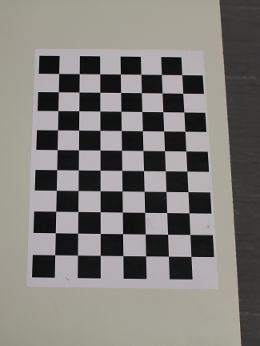
\includegraphics[scale=0.5]{chessboard_small}
		\caption{Kalibrierebene definiert durch Schachbrettmuster auf planarer Oberfläche}
		\label{fig.chesscalib}
	\end{center}
	%\vspace*{-8mm}
\end{figure}

Aus verschiedenen Lagen werden anschließend mit der Kamera Bilder des Musters aufgenommen. Dabei spielt es keine Rolle, ob die Lage der Kamera oder des Musters zwischen den Aufnahmen variiert wird. Zu beachten ist jedoch, dass das Muster in allen Aufnahmen vollständig im Bild abgebildet wird. Darüber hinaus sollten sowohl translatorische als auch rotatorische Veränderungen der Pose vorgenommen werden. Idealerweise liegen die Posen der aufgenommenen Perspektiven auf einer Halbkugel um die Kalibrierebene.\\

Die Kalibrierung erfordert die Bestimmung der Ebene des Musters mittels darauf befindlicher, eindeutig zu identifizierender Punkte. Das Schachbrettmuster eignet sich besonders als Kalibriermuster, da zwischen den Feldern ein hoher Kontrast besteht. Die Eckpunkte können somit robust erkannt und extrahiert werden, woraufhin sich die Kalibrierebene bestimmen lässt.\\

\prever{
%\red[\abb{fig.chessplane} Vielleicht chesscalib (b)!? Oder 3 verschiedene Posen mit Koordinatensystem!?]\\
}

Die vier intrinsischen und die sechs extrinsischen Parameter werden zunächst auf Basis des Lochkameramodells ohne Berücksichtigung der radialen Verzeichnungen bestimmt. Die Abbildung eines Punktes auf die Sensorebene kann unter Verwendung der intrinsischen und extrinsischen Kameramatrix nach \eq{eq.persp_abb} ausgedrückt werden als:
%
\begin{equation}
s \cdot 
\mat{c}{
u\\
v\\
1
}
=
\mat{cccc}{
f_x & 0 & u_\ind{0} & 0\\
0 & f_y & v_\ind{0} & 0\\
0 & 0 & 1 & 0
}
\cdot
\mat{ccc|c}{
  & \rmat{K}{0} &   & \ve{K}{t}_{\ind{0}} \\
\hline
0 &      0      & 0 & 1 \\
}
\cdot
\mat{c}{
X\\
Y\\
Z\\
1
}
\end{equation}

Eine Vereinfachung dieser Darstellung lässt sich erreichen, indem die Kalibrierebene mit der globalen Ebene in $Z=0$ gleichgesetzt wird. Dadurch können die Dimensionen der intrinsischen und extrinsischen Kameramatrix reduziert werden. Die Abbildungsgleichung ergibt sich damit unter Umformulierung der Rotations-Matrix als $\rmat{K}{0} = [\vec{r}_1 \quad \vec{r}_2 \quad \vec{r}_3]$ zu:

\nomenclature[l]{$\vec{r}_i$}{Vektor der $i$-ten Spalte der Rotationsmatrix}
%
\begin{equation}
s \cdot
\mat{c}{
u\\
v\\
1
}
 = 
\underbrace{
\mat{ccc}{ 
	f_x & 0 & u_\ind{0}\\
	0 & f_y & v_\ind{0}\\
	0 & 0 & 1
}
\cdot
\mat{ccc}{ 
	\vec{r}_1 & \vec{r}_2 & \ve{K}{t}_{\ind{0}} \\
}
}_{\vec{H}}
\cdot
\mat{c}{
	X\\
	Y\\
	1
}
\end{equation}

\nomenclature[l]{$\vec{H}$}{Homographie-Matrix}


Die $(3 \times 3)$ Matrix $\vec{H}$ wird als Homographie-Matrix bezeichnet und beschreibt die Abbildung zwischen den Punkten zweier Ebenen. Aufgrund des frei wählbaren Skalierungsfaktors $s$ besitzt die Homographie-Matrix bei neun Einträgen insgesamt acht Freiheitsgrade. Jeder detektierte Punkt des Musters liefert zwei Korrespondenzen. Aus vier Punkten ergeben sich damit acht Gleichungen, welche ein Gleichungssystem zur Bestimmung der Homographie-Matrix bilden.\\
%\red[ Homographie beschreibt Transformation eines Quadrilaterals, damit würde auch die Bestimmung von mehr als vier Punkten keine zusätzlichen Informationen liefern.]\\

Da die Betrachtung des Musters aus verschiedenen Perspektiven erfolgt, müssen zunächst für jede Aufnahme die sechs räumlichen Freiheitsgrade bestimmt werden. Es verbleiben damit jeweils zwei Parameter zur Bestimmung der intrinsischen Parameter. Da die intrinsische Kameramatrix nach \eq{eq.intrinsic} vier Freiheitsgrade besitzt, werden $n = 2$ Aufnahmen benötigt um die intrinsischen Parameter eindeutig festlegen zu können. In der Praxis sollten jedoch $n \geq 10$ Aufnahmen verwendet werden, um numerische Stabilität der Lösung zu gewährleisten und Messrauschen zu kompensieren \cite{Bradsky2008}.\\

%Homographie bildet 2D auf 2D ab; Gesamtabbildung angeben, reduzieren durch z = 0; Homographiematrix aufstellen; Anzahl freier Parameter nennen (8) -> mindestens 2 Aufnahmen erforderlich; Besser mehr als 10; \red[Formeln!?]; Verweis auf Lösung reicht eigentlich, Parameter können damit bestimmt werden; Dann weiter zur Bestimmung der (radialen) Verzeichnungsparameter.
%Obwohl theoretisch $n = 2$ Aufnahmen für eine eindeutige Lösung ausreichend sind, sollten für eine robuste Bestimmung der Parameter insgesamt $n \geq 10$ Bilder aufgezeichnet werden \cite{Bradsky2008}.\\

Basierend auf den ermittelten intrinsischen Parametern können nun die radialen Verzeichnungsparameter angenähert werden. Unter der Annahme, dass die radiale Verzeichnung klein ist, kann davon ausgegangen werden, dass die intrinsischen Parameter bereits hinreichend genau bestimmt wurden. Die ermittelten Werte können damit als initale Approximation verwendet werden, um die Verzeichnungsparameter zu bestimmen. In einem abschließenden Optimierungsschritt werden alle ermittelten Parameter verfeinert. Dazu erfolgt eine Minimierung der Fehler zwischen den aufgenommenen und den auf Basis des ermittelten Modells bestimmten Pixelwerten des Musters.

%Es erfolgt eine Verfeinerung der Parameter durch Minimierung der \red[GLEICHUNG!?].%


%\red[Vereinfachung später, dass T-WELT = T-0]
%Kalibrierung der Kamera
%Kameramatrix aufführen, Herleitung ist aber nicht wirklich relevant. Extrinsische und intrinsische Transformation unterscheiden. Parameter beschreiben und erklären. Lochkameramodell als Grundlage nennen und in ein paar Sätzen erläutern, aber nicht zu detailliert drauf eingehen. Ermittlung der Tiefeninformationen beschreiben. projektor als inverse Kamera.\\

\prever{
%\red[Kalibrierung der Kameras (RGB + IR) mit cameracalibration beschreiben und Gesamtsystem mit Matlab box bouguet (gibt extr. und intr. parameter).\\
%Isometrische Ansicht als Prinzip der Kalibrierung? Schachbrett fest und 3 Ansichten des Systems (der Kamera) mit Koordinatensystemen!?\\]
}

\subsection{Projektorkalibrierung}
\label{chap.projcalib}
Um die Darstellung visueller Informationen an definierten Stellen im Raum zu ermöglichen ist eine Kalibrierung des Projektors erforderlich. Indem die Projektion in umgekehrter Richtung betrachtet wird, kann ein Projektor, wie in \kapitel{chap.kinect} erwähnt, als inverse Kamera aufgefasst werden. Das Verfahren zur Kamera-Kalibrierung lässt sich dadurch auf den Projektor erweitern \cite{Falcao2008}.\\

Aufgrund der Fixierung des Projektors im \kps{} ist die Lage bezüglich des Kamera-Koordinatensystems unveränderlich. Anstelle einer globalen Positionsbestimmung ist daher insbesondere die Ermittlung der konstanten, relativen Transformation zwischen den Koordinatensystemen des Projektors und der Kamera von Interesse. Ziel der Kalibrierung des Projektors ist daher die Bestimmung der konstanten Parameter der intrinsischen Projektormatrix und der Pose des Projektors bezüglich des Kamera-Koordinatensystems $\ks{K}$.\\

Die Kalibrierung erfolgt anhand des von Falcao \textit{et al.} beschriebenen Verfahrens \cite{Falcao2008}. Dabei wird zur Definition der Kalibrierebene erneut ein Muster auf einer Platte verwendet. Ein weiteres Kalibriermuster wird als digitales Bild erstellt und wie in \abb{fig.projcalib} gezeigt durch den Projektor neben das reale Muster auf die Platte projiziert.

\clearpage{}

\begin{figure}[ht]
	\begin{center}
		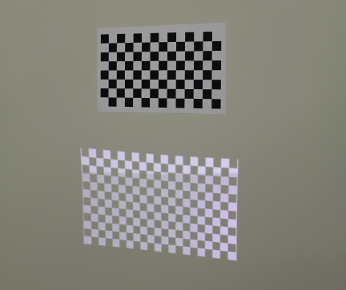
\includegraphics[scale=0.5]{chessboard_projected_small_cropped}
		\caption{Reales und projiziertes Schachbrettmuster zur Kalibrierung des Projektors}
		\label{fig.projcalib}
	\end{center}
	%\vspace*{-8mm}
\end{figure}

\prever{
%\red[Bild 90 grad rotieren\\]
}

Um die gemeinsame Kalibrierebene zu bestimmen ist die Aufnahme beider Muster in einem Bild erforderlich. Da die Kalibrierung auch die Transformation zwischen den Koordinatensystemen von Kamera und Projektor bestimmen soll, werden die Muster mit der zuvor kalibrierten Kamera des Systems aufgezeichnet.\\

Zunächst ist es erforderlich, die Lage der Kamera bezüglich der Kalibrierebene zu ermitteln. Mit Hilfe der ermittelten intrinsischen Kameraparameter können die inertialen Koordinaten der Eckpunkte und die aufgespannte Ebene des realen Schachbretts leicht bestimmt werden. Die Pixel-Koordinaten des projizierten Musters können ebenfalls extrahiert werden. Da die Kalibrierebene bekannt ist, kann der in \eq{eq.persp_abb} eingeführte Skalierungsfaktor in den Abbildungsgleichungen bestimmt und somit die räumliche Position der projizierten Eckpunkte ermittelt werden.\\

Es liegen nun wie bei der Kamerakalibrierung Korrespondenzen zwischen den Punkten in der Kalibrierebene und der gedachten Sensorebene des Projektors vor. Damit ist das bereits beschrieben Kalibrierverfahren nach Zhang anwendbar, wodurch die intrinsische Projektormatrix $\tmat{SP}{P}$ bestimmt werden kann.\\

\prever{
%\red[Auch hier isometrische Ansicht mit Gesamtsystem? Transformationen lassen sich dort gut zeigen\\]
}

Da für jede Aufnahme während der Kalibrierungsvorgänge die Transformationen zwischen dem Inertialkoordinatensystem und den Koordinatensystemen von Kamera und Projektor ermittelt wurden, kann die statische Transformation zwischen Kamera und Projektor ebenfalls bestimmt werden:
%
\begin{equation}
\tmat{K}{P} = \left( \tmat{0}{K} \right)^{-1} \cdot \tmat{0}{P} = \tmat{K}{0} \cdot \tmat{0}{P}
\end{equation}

Da das \kps{} damit als Gesamtsystem kalibriert ist, wird ein gemeinsames Basis-Koordinatensystem $\ks{KPS}$ definiert. Dieses unveränderliche Koordinatensystem dient als Referenz, um die externen Transformationen zu beschreiben. Die Orientierung wird entsprechend der ($z$,$y'$,$x''$)-Konvention gewählt und die Position wie in \abb{fig.coords_kps} dargestellt in Abhängigkeit der Kinect definiert. Die Transformation $\tmat{KPS}{K}$ ergibt sich damit aus den geometrischen Beziehungen, woraufhin sich $\tmat{KPS}{P}$ ebenfalls bestimmen lässt.


\begin{figure}[ht]
	\begin{center}%
		\includesvgnew[1]{images/coordinates_kps}%
		%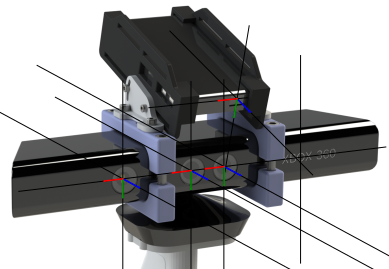
\includegraphics[scale=1.0]{coordinate_systems}
		\caption{Basis-Koordinatensystem des \kps{s}}
		\label{fig.coords_kps}
	\end{center}
	%\vspace*{-8mm}
\end{figure}

\prever{
%\red[
%Notation\\
%Lochkameramodell\\
%Intrinsische + Extrinsische Parameter\\
%Kalibrierung Kamera (RGB+IR)\\
%Stereosystem Kinect (Epipolargeometrie etc.), Prinzip kurz erläutern, Buch und Davids Arbeit - Weiter vorne schon?\\
%Projektor als inverse Kamera\\
%Kalibrierung Projektor + Kamera+Projektor\\
%Projektor Linsenverzeichnung!?\\
Toolboxen und verwendete Kalibrierungsnode nennen?\\
%Transformationen zwischen den Koordinatensystemen angeben wenn möglich (oder in Kapiteln erst?)]\\
}

%\red[Gemeinsames Koordinatensystem des Gesamtsystems definieren, über welches die Lage in der Umgebung beschrieben wird. $\ks{KPS}$\\]

%\red[Wichtig sind die Transformationen zwischen den Koordinatensystemen und die Abbildung des Projektors. Die Transformation erfolgt allerdings immer über die Kamera, da diese im Weltkoordinatensystem lokalisiert wird. Für die Kalibrierung sind die intrinsischen und extrinsischen Parameter relevant, aber auch die Herkunft?\\]

\prever{
%\red[Transformationen:\\
%Map = World\\
%World -> BaseLink -> CameraLink -> Camera\\
%Camera -> Projector\\
%Projector -> IntrinsicProj\\
%World -> Objects\\
%World -> ARMarker (eq. to Objects)\\
%]
}

\section{Verwendete Softwarebibliotheken}
%\red[GUI auslagern als eigenen Punkt!?\\]
Zur Realisierung der einzelnen Systemfunktionen wurden Komponenten erstellt, welche auf verschiedenen Softwarebibliotheken aufbauen.
Im Anschluss an die Vorstellung der verwendeten Bibliotheken und Softwareumgebungen wird die erstellte Programmstruktur beschrieben, welche die verschiedenen Funktionsbereiche des \kps{s} abbildet.
%Bevor die Programmstruktur näher erläutert wird, sollen deshalb zunächst die verwendeten Bibliotheken und Softwareumgebungen dargestellt werden.
%Anschließend erfolgt eine Beschreibung der erstellten Programmstruktur und der innerhalb einer grafischen Benutzeroberfläche zusammengefassten Bedienfunktionen des Systems.

\subsection{Robot Operating System}
\label{chap:ros}
Das Robot Operating System (ROS) ist eine speziell für die Anwendung in der Robotik entwickelte, quelloffene Sammlung aus Softwarebibliotheken \cite{ROS}. Neben Treibern für verschiedene Hardwarekomponenten und speziellen Algorithmen bietet ROS eine Umgebung, welche die Integration von und Kommunikation zwischen verschiedenen Modulen vereinfacht, um komplexe und robuste Anwendungen zu realisieren. Die in dieser Arbeit entwickelte und verwendete Software wurde für die ROS-Distribution Indigo optimiert.

\nomenclature[a]{ROS}{Robot Operating System}

\subsection{Open Source Computer Vision Library}
Die Open Source Computer Vision Library (OpenCV) ist eine quelloffene Bibliothek aus Funktionen und Algorithmen zur Anwendung in der Bild- und Videoverarbeitung \cite{OpenCV}. Nachdem OpenCV ursprünglich von einer Forschungsgruppe bei Intel (Intel Corporation, Santa Clara, USA) entwickelt wurde \cite{Laganiere2011}, wird die Bibliothek heute von einer großen Anzahl an Firmen und Entwicklern verwendet und ständig weiterentwickelt. Sie umfasst mittlerweile mehr als \SI{2500}{} optimierte Algorithmen zur Anwendung in Bereichen wie Objekterkennung, Segmentierung oder Navigation. Im Rahmen dieser Arbeit wird die Version 2.4.8 der Bibliothek eingesetzt.

\nomenclature[a]{OpenCV}{Open Source Computer Vision Library}

\subsection{Point Cloud Library}
Die Struktur von Punktwolken wird verwendet, um die von der Kinect aufgenommenen Tiefeninformationen darzustellen und weiterverarbeiten zu können. Die Point Cloud Library (PCL) wurde mit dem Ziel entwickelt, ein Rahmenwerk zu schaffen, welches die Verarbeitung von Punktwolken mittels verschiedener Algorithmen ermöglicht. Ähnlich wie OpenCV für die 2D-Bildverarbeitung wird PCL bezogen auf Punktwolken in den Bereichen Objekterkennung, Segmentierung oder Filterung angewendet. Auch PCL ist eine quelloffene Bibliothek, welche von einer Vielzahl an Firmen und Entwicklern ständig überarbeitet und erweitert wird \cite{PCL}. PCL wird in dieser Arbeit in der Version 1.7.1 verwendet um die Visualisierung und Verarbeitung der durch die Kinect ermittelten Punktwolken zu ermöglichen.

\nomenclature[a]{PCL}{Point Cloud Library}

\subsection{Qt}
Die von der Firma Digia (Digia Plc, Helsinki, Finnland) verwaltete Qt Bibliothek ermöglicht eine plattformunabhängige Entwicklung von grafischen Benutzerschnittstellen im C++ Standard \cite{Qt}. Die Qt Bibliothek in der Version 5.2.1 wird in dieser Arbeit verwendet, um die Schnittstelle zu realisieren, mit welcher der Benutzer Zugriff auf die Funktionen der verschiedenen Programmkomponenten erhält.

\subsection{Visualization Toolkit}
\label{chap.vtk}
Das Visualization Toolkit (VTK) stellt eine auf dem C++ Standard basierende Bibliothek dar, welche für die Verarbeitung und Visualisierung von 3D-Bilddaten entwickelt wurde. Die Firma Kitware (Kitware Inc., New York, USA) entwickelt die Bibliothek ständig weiter und stellt sie als quelloffene Software zur Verfügung \cite{VTK}. Verschiedene Schnittstellen zwischen VTK und PCL ermöglichen neben der Darstellung von 3D-Objekten auch die Integration und Visualisierung von Punktwolken. Die Verfahren zur Abbildung dreidimensionaler Szenen werden im Rahmen dieser Arbeit genutzt, um die Modellumgebung zu visualisieren und die perspektivisch korrekte Projektion zu generieren. Dabei wird die VTK Version 5.8.0 eingesetzt.

\nomenclature[a]{VTK}{Visualization Toolkit}

\prever{
%\red[Ausführlicher?\\]
%\red[Versionen!\\]
}

\prever{
%\red[\subsection{Programmstruktur}]
}
\section{Softwarestruktur}
\label{chap.softwarestruct}
%\red[Mit aufnehmen in dieser Liste? Oder ganz am Ende (nach Interaktion) Komplettes GUI und alle Transformationen zusammenfassen?\\]%
Die für die Anwendung des \kps{s} als selbstlokalisierendes, handgeführtes Projektionssystem entwickelte Software umfasst verschiedene Module, welche durch ROS verknüpft werden. Dies ermöglicht den Informationsaustausch zwischen den Komponenten auf Basis definierter Daten- und Kommunikationsstrukturen. Der Austausch einzelner Komponenten ist damit jederzeit möglich, sodass die Entwicklung und Integration optimierter Module je nach Anwendungsgebiet vorgenommen werden kann. Die Entwicklung und Ausführung der Software erfolgte auf einem PC mit dem Linux basierten Betriebssystem Ubuntu. Als Entwicklungsumgebung wurde Qt Creator gewählt, welche insbesondere auf die Entwicklung von plattformunabhängigen Programmen mit der Qt Bibliothek in der Programmiersprache C++ ausgelegt ist.
Einen Überblick über die Softwaremodule, ihre Verknüpfung untereinander und die Beziehungen zur realen und modellierten Umgebung zeigt Abbildung \ref{fig.modules}.\\

\begin{figure}[ht]
	\begin{center}%
		\includesvgnew[1]{images/modules_solo_02}%
		\caption{Übersicht über die Verknüpfungen zwischen Datenstruktur, Softwaremodulen und Umgebung}
		\label{fig.modules}
	\end{center}
	%\vspace*{-8mm}
\end{figure}

\prever{
%\red[Modelldaten an Überschrift von Kapitel 4 anpassen! Datengrundlage/Datenbasis/Modelldaten. Und gesondert darstellen (andere Farbe+Form)\\]
%\red[handgeführtes ersetzen durch handführbares?\\]
}

Die Datengrundlage stellt die Repräsentation der Umgebung und der virtuellen Modelle dar. Das Modul \textit{Lokalisation} umfasst die Implementierungen zur Bestimmung der Pose des \kps{s} innerhalb der realen Umgebung. Es empfängt die Farb- und Tiefeninformationen der Kameras der Kinect sowie die Orientierungsinformationen der IMU und ermittelt durch den Abgleich mit der Modellumgebung die aktuelle Systempose. Definiert wird die Pose dabei durch den Benutzer über Bewegung des \kps{s}. Die kontinuierlich bestimmte Pose wird an das Modul \textit{Visualisierung} übertragen, welches daraufhin die Lage des \kps{s} innerhalb der Modellumgebung ermittelt. Durch Bestimmung der perspektivischen Abbildung ausgewählter Modelldaten wird anschließend die Projektorsicht simuliert und dem Benutzer über das \kps{} durch Projektion visualisiert.\\ 

%Dazu werden im Modul \textit{Visualisierung} alle Transformationen bestimmt, welche die Pose  der Modellumgebung definieren.\\
Das Modul \textit{Interaktion} ermöglicht dem Benutzer die Modifikation der visualisierten Modelldaten indem die Tiefeninformationen der Kinect ausgewertet werden. Die Befehle des Benutzers können so erkannt und anschließend an das Modul \textit{Visualisierung} übertragen werden. Durch die Rückkopplung zu den Modelldaten können diese daraufhin angepasst werden. Das Modul \textit{Visualisierung} integriert die Benutzerinteraktion in die Darstellung der Modelldaten, so dass eine visuelle Rückmeldung während der Interaktion erfolgt.\\

Darüber hinaus wurde eine grafische Benutzeroberfläche (GUI) implementiert, welche verschiedene Konfigurationsmöglichkeiten bietet. Sie ermöglicht dem Benutzer direkten Zugriff auf die Einstellungen der Module. Diese übergeordnete Kommunikationsstruktur wurde in der Übersicht nicht explizit aufgeführt, da die Anwendung unabhängig von der Bedienung der Benutzeroberfläche lauffähig ist.\\

\nomenclature[a]{GUI}{Graphical User Interface}

In den folgenden Kapiteln wird zunächst die Datengrundlage spezifiziert und darauf aufbauend werden die Struktur und Funktionalität der beschriebenen Softwaremodule erläutert.\\
\prever{
\red[Satz ist kein Absatz!\\]
}


\prever{
%\red[eigene leistung]
}

\prever{
%\red[In den folgenden Kapiteln erfolgt eine Spezifizierung der Module und ihrer Komponenten.\\]
%\red[Wie KPS, Benutzer und Modelldaten bezeichnen?\\]
}

%Module: \mLocalization - EKF Odometrie (Tracking) - Visuelle Odometrie - IMU - Visualisierung - Transformation - Interaktion - Benutzeroberfläche - Projektion - Kartenserver\\

%Das \mLocalization bestimmt und überwacht die aktuelle Position des \kps{s}. Es ermittelt die initiale Position mittels globaler Lokalisation auf Basis der vom \mMapserver zur Verfügung gestellten Karte. Als weitere Eingangsgröße verwendet es die Odometriedaten, welche vom \mEkf zur Verfügung gestellt werden um Veränderungen in der Position während der Bedienung zu erkennen und die Positionsdaten dementsprechend zu aktualisieren. Das \mEkf selbst verwendet und filtert dabei die visuellen Odometriedaten des \mFovis und die Lagedaten des \mImu \red[TODO Moduls] um die kombinierten Odometriedaten zu bestimmen.\\
%Diese so vom \mLocalization bestimmten Positionsdaten werden dem \mTransformation übermittelt, welches alle Koordinatentransformationen zwischen der ermittelten Kameraposition, dem Projektor und den relevanten Objekten der Umgebung berechnet. Diese Berechnungen werden dann vom \mVisualization verwendet, um ein Abbild der aktuellen Projektorsicht innerhalb der 3D Umgebung zu erstellen. Dem Benutzer wird diese Ansicht anschließend sowohl über die Benutzeroberfläche durch das \mGui als auch über die Projektion durch das \mProjection dargestellt. \\
%Das \mInteraction erkennt vom Benutzer durchgeführte Gesten oder Bewegungen, über welche er auf Basis der projizierten Daten mit der Modellumgebung interagiert. Die Steuerungsbefehle werden dann über das \mTransformation an das \mVisualization übertragen, wo diese interpretiert werden und in Form von Modifikationen der Modellumgebung umgesetzt werden.\\
%Die jeweilige Realisierung der Module wird in den folgenden Kapiteln näher spezifiziert.\\


\prever{
%\red[Buttons eingebaut, hier als Möglichkeit der Interaktion erwähnen(?)- Aber welches Modul managed das?]
}
